\subsection{Internet of Things}
\begin{frame}
 \frametitle{\textit{Internet of Things}}

 \begin{itemize}
  \item<1-> Tecnologia diffusasi recentemente
  \item<2-> Necessit\`a di sincronizzare \\ informazioni in un ambiente
distribuito
  \item<3-> Blockchain come soluzione
 \end{itemize}

 \begin{textblock*}{5cm}(8.5cm,2.5cm)
  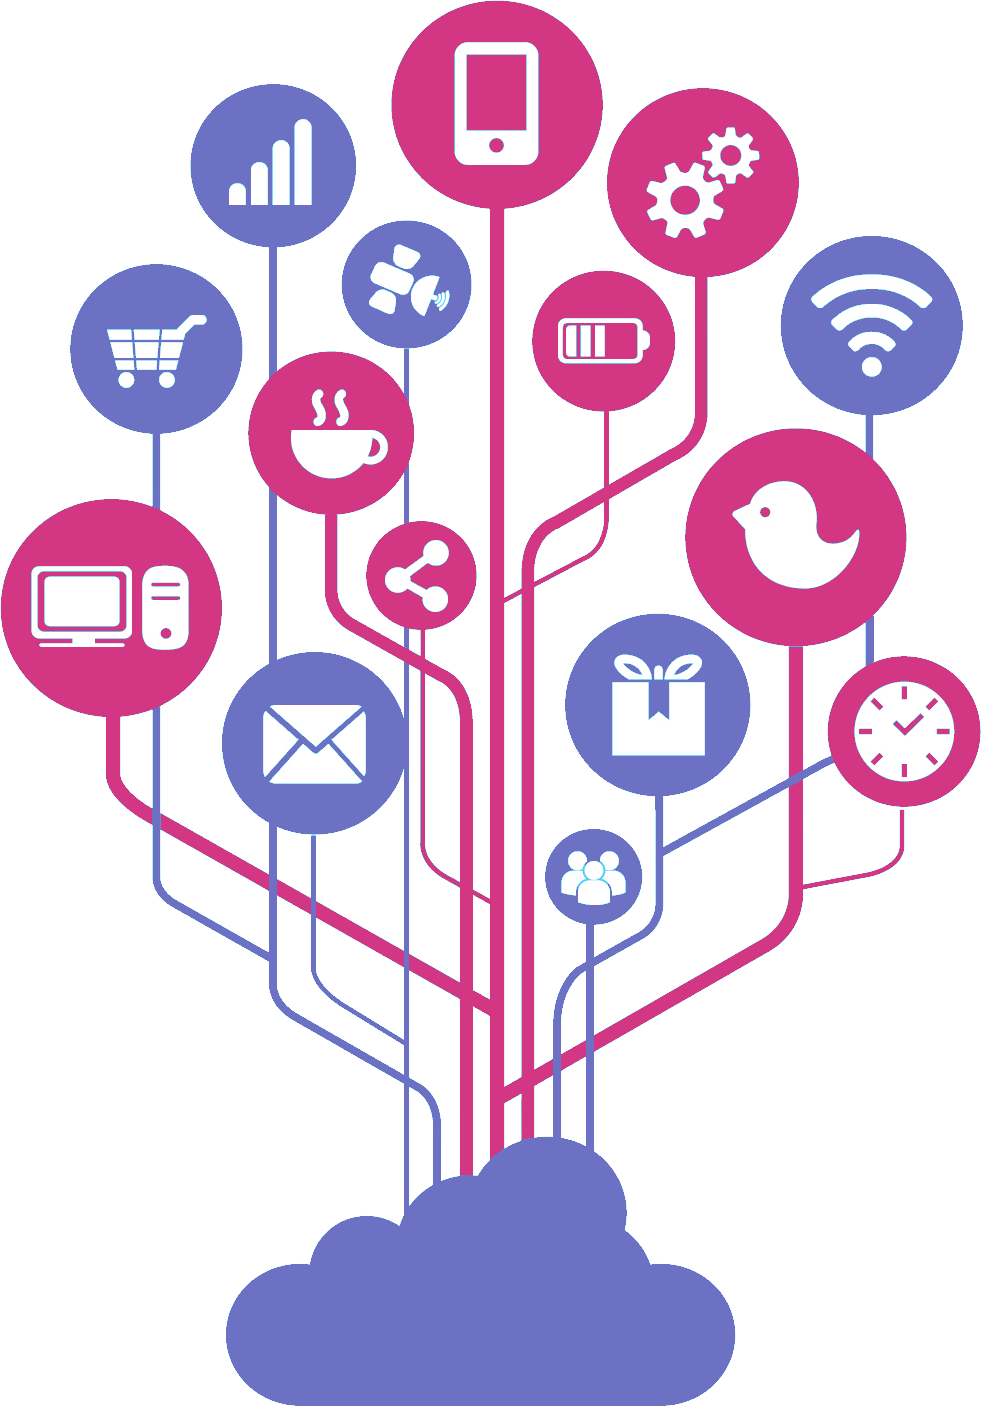
\includegraphics[scale=0.2]{Iot1}
 \end{textblock*}

\end{frame}

\begin{frame}
 \frametitle{\textit{Internet of Things}}

 \begin{itemize}
  \item<1-> Vantaggi:
  \begin{itemize}
   \item Nessun server centrale
   \item Nessun database centrale a cui trasmettere dati
   \item Maggiore tolleranza a problemi di rete
  \end{itemize}

  \item<2-> Svantaggi:
  \begin{itemize}
   \item \textit{Trust issues}
   \item Algoritmo di mining per la concatenzione dei blocchi
  \end{itemize}

 \end{itemize}


 \begin{textblock*}{5cm}(7cm,2cm)
  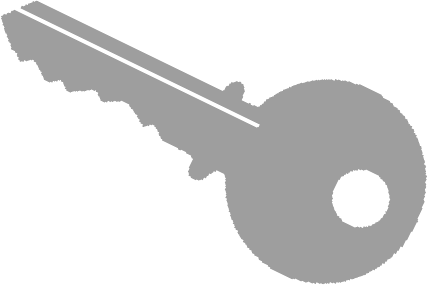
\includegraphics[scale=0.1]{key}
 \end{textblock*}


 \begin{textblock*}{5cm}(2cm,7cm)
  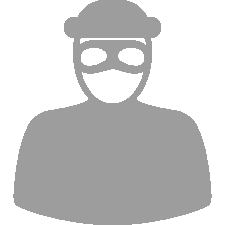
\includegraphics[scale=0.2]{robber}
 \end{textblock*}

\end{frame}
